\section{Main page}

The overhall principle of the main Page of mycustom is resumed on Figure \ref{fig:principe}. The main page of the website is organized as a single app page. 

In order to soft code (i.e to let the website manager change things without having to rewrite some peaces of code) the visual aspect of the main page, the characteristics of the website parts are stored in the database. The link between the database and the interface client is done by several Django App namely \texttt{"home", "collection$\_$ephemere", "cutsomise", "achetez", "vendre"}. These apps contains the HTML templates that render in the interface client and the Django models used to fulfill them. The interface admin is able to modify the database in the backend and thus, the interface client. In order to fully understand how a Django app works, see \cite{Django, Django_doc}. 

\begin{figure}[!ht]
	\centering
	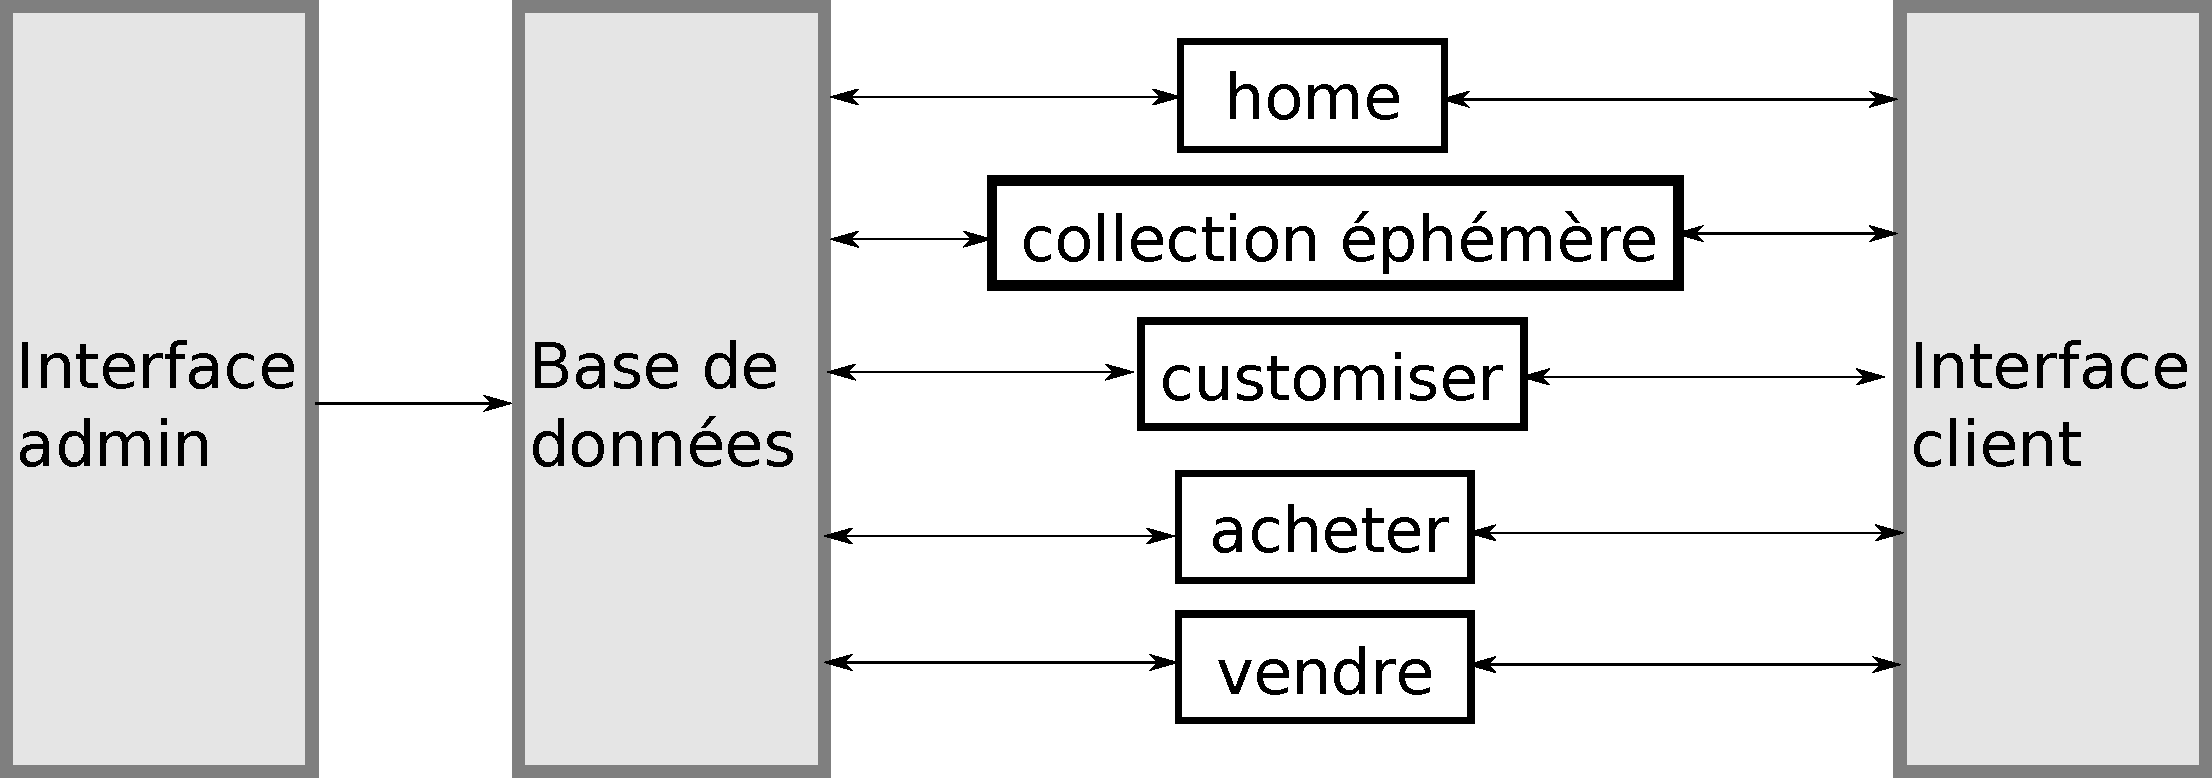
\includegraphics[width=0.45\textwidth]{mainPage/principe}
	\caption{Global principle of the mycustom website}
	\label{fig:principe}
\end{figure}

The purpose of each of theses section is the following : 

\begin{itemize}
	\item \texttt{home} : Contains the landing page of the website, i.e the first thing that the client see. The Django app contains a video for the welcome page, the HTML template for the header, the footer, the menu and the welcome page. The Django models contains all the visual characteristic for the welcome page. Again, in order to fully understand a Django model, see \cite{Django, Django_doc}.
	\item \texttt{collection$\_$epehemere} : Contains the transitory trends, i.e  the textile and logo of the month. 
	\item \texttt{customiser} : This is the place where the customer choose a textile. The textile are classed by two manners : by category and by type of product. 
	\item \texttt{achetez} : This the section where the customer choose a product by logo
	\item \texttt{vendre} : this is the place where a customer can signe in/up. The social media aspect of mycsutom needs to be put in this section. 
\end{itemize}

In order to be more specific, the web manager can modify the aspect of the website by using the admin interface. He can input some images or data that will be stored in the data base and then render on the front page.

The Bootstrap framework is used in order to render the visual aspects of the website. In order to fully understand Bootstrap see \cite{Bootstrap, Bootstrap_doc}. The Django template engine will fill in Bootstrap code with data of the database in order to achieve the desire visual output. 



 


